```latex
\chapter{Công nghệ và phiên bản}
\label{chap:technologies}

\section{Nguồn xác định phiên bản}

Phiên bản công nghệ chỉ được ghi nhận khi có thể đối chiếu từ manifest,
project file hoặc lock file trong repository.

\textit{Constraint} biểu thị khoảng phiên bản mà manifest cho phép, trong khi
\textit{locked version} là phiên bản dependency đã được khóa trong checkout.
Việc một dependency xuất hiện trong lock file chỉ xác nhận trạng thái
\textit{Configured}, không chứng minh môi trường runtime đang sử dụng đúng
phiên bản đó.

\begingroup
\small
\renewcommand{\arraystretch}{1.15}
\setlength{\tabcolsep}{4pt}

\begin{longtable}{
    >{\raggedright\arraybackslash}p{0.17\textwidth}
    >{\raggedright\arraybackslash}p{0.19\textwidth}
    >{\raggedright\arraybackslash}p{0.17\textwidth}
    >{\raggedright\arraybackslash}p{0.27\textwidth}
    >{\centering\arraybackslash}p{0.12\textwidth}
}

\caption{Công nghệ và phiên bản được xác định từ repository}
\label{tab:technology-versions}\\

\hline
\rowcolor{gray!15}
\textbf{Phạm vi} &
\textbf{Công nghệ} &
\textbf{Phiên bản} &
\textbf{Nguồn xác định} &
\textbf{Trạng thái} \\
\hline
\endfirsthead

\hline
\rowcolor{gray!15}
\textbf{Phạm vi} &
\textbf{Công nghệ} &
\textbf{Phiên bản} &
\textbf{Nguồn xác định} &
\textbf{Trạng thái} \\
\hline
\endhead

Firmware / simulator &
C++ standard &
GNU C++17 &
Hai file \path|platformio.ini| &
Configured
\\

Firmware / simulator &
ArduinoJson &
Constraint \texttt{\string^7.0.4} &
\path|platformio.ini| &
Configured
\\

Firmware / simulator &
PubSubClient &
Constraint \texttt{\string^2.8} &
\path|platformio.ini| &
Configured
\\

Firmware / simulator &
PlatformIO platform \texttt{espressif32} &
Không khóa phiên bản &
\path|platformio.ini| &
Not Found
\\

Device Monitor &
PHP &
Constraint \texttt{\string^8.1} &
\path|composer.json| &
Configured
\\

Device Monitor &
Slim &
4.15.2 &
\path|composer.lock|; constraint \texttt{\string^4.14} &
Configured
\\

Device Monitor &
Slim PSR-7 &
1.8.0 &
\path|composer.lock|; constraint \texttt{\string^1.7} &
Configured
\\

SmartWater Admin &
PHP &
Constraint \texttt{\string^8.3} &
\path|composer.json| &
Configured
\\

SmartWater Admin &
Laravel Framework &
13.18.1 &
\path|composer.lock|; constraint \texttt{\string^13.8} &
Configured
\\

SmartWater Admin &
Laravel Tinker &
3.0.2 &
\path|composer.lock|; constraint \texttt{\string^3.0} &
Configured
\\

Admin assets &
Vite &
8.1.5 &
\path|package-lock.json|; constraint \texttt{\string^8.0.0} &
Configured
\\

Admin assets &
Tailwind CSS &
4.3.3 &
\path|package-lock.json|; constraint \texttt{\string^4.0.0} &
Configured
\\

Admin assets &
Tailwind Vite plugin &
4.3.3 &
\path|package-lock.json| &
Configured
\\

Admin assets &
Laravel Vite plugin &
3.1.3 &
\path|package-lock.json| &
Configured
\\

Admin UI/CDN &
Bootstrap &
5.3.3 &
\path|resources/views/layouts/app.blade.php|;
\path|auth/login.blade.php| &
Configured
\\

Admin UI/CDN &
Bootstrap Icons &
1.11.3 &
\path|resources/views/layouts/app.blade.php|;
\path|auth/login.blade.php| &
Configured
\\

Admin UI/CDN &
jQuery &
3.7.1 &
\path|resources/views/layouts/app.blade.php| &
Configured
\\

Admin UI/CDN &
DataTables &
1.13.8 &
\path|resources/views/layouts/app.blade.php| &
Configured
\\

Admin UI/CDN &
ApexCharts &
3.49.1 &
\path|resources/views/layouts/app.blade.php| &
Configured
\\

Worker &
.NET target framework &
\texttt{net8.0} &
\path|SmartWater.MqttService.csproj| &
Configured
\\

Worker &
MQTTnet &
4.3.7.1207 &
\path|SmartWater.MqttService.csproj| &
Configured
\\

Worker &
Dapper &
2.1.28 &
\path|SmartWater.MqttService.csproj| &
Configured
\\

Worker &
MySqlConnector &
2.3.7 &
\path|SmartWater.MqttService.csproj| &
Configured
\\

Worker &
Hosting / Windows Services &
8.0.1 / 8.0.0 &
\path|SmartWater.MqttService.csproj| &
Configured
\\

Persistence &
MySQL Server &
Không xác định &
Không có server manifest hoặc image tag &
Not Found
\\

Broker &
HiveMQ Server &
Không xác định &
Không có broker manifest hoặc image tag &
Not Found
\\

\hline
\end{longtable}
\endgroup

\section{Vai trò của các công nghệ}

Technology stack của hệ thống được chia thành năm phạm vi chính: firmware,
message broker, Device Monitor, SmartWater Admin và worker nền. Mỗi nhóm công
nghệ đảm nhiệm một vai trò riêng trong luồng thu thập, truyền tải, xử lý, lưu
trữ và hiển thị dữ liệu.

\subsection{Firmware và ESP32 Simulator}

Firmware và simulator được xây dựng bằng C++ trên nền tảng PlatformIO và
Arduino framework. Nhóm công nghệ này thực hiện các chức năng gần thiết bị,
bao gồm:

\begin{itemize}
    \item khởi tạo kết nối Wi-Fi của ESP32;
    \item thiết lập kết nối đến HiveMQ thông qua giao thức MQTT;
    \item đọc hoặc mô phỏng dữ liệu telemetry;
    \item xây dựng payload trước khi gửi lên broker;
    \item publish dữ liệu theo topic đã được cấu hình;
    \item xử lý trạng thái kết nối và thực hiện reconnect khi cần thiết.
\end{itemize}

\textbf{PlatformIO} quản lý cấu hình build, board, compiler và dependency của
firmware. Chuẩn GNU C++17 được sử dụng để biên dịch mã nguồn cho ESP32.

\textbf{ArduinoJson} chịu trách nhiệm tạo và phân tích payload JSON. Thư viện
này được sử dụng để chuyển dữ liệu nội bộ của firmware thành message có cấu
trúc trước khi publish qua MQTT.

\textbf{PubSubClient} cung cấp MQTT client cho ESP32, bao gồm kết nối broker,
publish message, subscribe topic và duy trì trạng thái kết nối MQTT.

ESP32 Simulator sử dụng cùng nhóm công nghệ để mô phỏng luồng gửi telemetry
mà không phụ thuộc hoàn toàn vào phần cứng và cảm biến thực tế.

\subsection{HiveMQ Broker}

HiveMQ đóng vai trò message broker trung gian giữa thiết bị và các thành phần
tiêu thụ dữ liệu.

Broker thực hiện các chức năng chính sau:

\begin{itemize}
    \item tiếp nhận message được publish từ ESP32 hoặc simulator;
    \item phân phối message đến các client đã subscribe đúng topic;
    \item tách biệt thiết bị gửi dữ liệu khỏi ứng dụng xử lý dữ liệu;
    \item hỗ trợ nhiều client cùng publish hoặc subscribe;
    \item cung cấp kết nối MQTT qua TLS và MQTT over WebSocket.
\end{itemize}

Firmware sử dụng kết nối MQTT qua TLS, trong khi giao diện Device Monitor sử
dụng MQTT over WebSocket để nhận message trực tiếp từ trình duyệt.

Repository không chứa broker manifest hoặc image tag, do đó phiên bản HiveMQ
Server không được xác định trong tài liệu.

\subsection{Device Monitor}

Device Monitor là thành phần tiếp nhận, kiểm tra và lưu trữ telemetry trước khi
dữ liệu được sử dụng bởi SmartWater Admin.

Backend của Device Monitor được xây dựng bằng PHP và Slim Framework. Slim cung
cấp lớp HTTP nhẹ để tổ chức route và xử lý request mà không cần sử dụng một
framework web đầy đủ.

Các chức năng chính của Device Monitor gồm:

\begin{itemize}
    \item cung cấp giao diện theo dõi kết nối MQTT;
    \item subscribe các topic telemetry thông qua HiveMQ;
    \item tiếp nhận payload từ MQTT client chạy trong trình duyệt;
    \item gửi payload đến HTTP endpoint của Device Monitor;
    \item parse và kiểm tra cấu trúc dữ liệu nhận được;
    \item chuẩn hóa dữ liệu telemetry trước khi ghi vào database;
    \item kiểm tra định danh MCU;
    \item cung cấp endpoint health cơ bản;
    \item trả kết quả xử lý cho giao diện giám sát.
\end{itemize}

\textbf{Slim PSR-7} cung cấp implementation cho HTTP request, response và stream
theo chuẩn PSR-7. Nhờ đó, các endpoint của Device Monitor có thể tiếp nhận JSON,
trả response và xử lý lỗi theo một interface thống nhất.

\textbf{PDO} được sử dụng để kết nối MySQL và thực thi các truy vấn persistence,
bao gồm kiểm tra MCU và ghi bản ghi telemetry.

\textbf{mqtt.js} chạy phía trình duyệt, kết nối HiveMQ qua WebSocket và chuyển
message nhận được đến backend Device Monitor. Phiên bản mqtt.js không được ghi
nhận vì module này không có \path|package.json| hoặc lock file riêng trong phạm
vi khảo sát.

\subsection{SmartWater Admin}

SmartWater Admin là ứng dụng quản lý nghiệp vụ và khai thác dữ liệu của hệ
thống. Ứng dụng được xây dựng bằng PHP và Laravel Framework.

Laravel đảm nhiệm các chức năng backend chính:

\begin{itemize}
    \item định nghĩa web route và API route;
    \item xử lý request thông qua controller;
    \item kiểm tra dữ liệu đầu vào bằng validation và Form Request;
    \item quản lý đăng nhập và session;
    \item ánh xạ dữ liệu database thông qua Eloquent ORM;
    \item tổ chức nghiệp vụ thông qua controller và service;
    \item tạo và quản lý schema bằng migration;
    \item render giao diện phía server bằng Blade template.
\end{itemize}

Trong phạm vi nghiệp vụ SmartWater, ứng dụng Admin hỗ trợ quản lý các nhóm dữ
liệu như:

\begin{itemize}
    \item người dùng và nhân viên;
    \item khách hàng;
    \item hợp đồng;
    \item sản phẩm và danh mục;
    \item kho và lô hàng;
    \item thiết bị và MCU;
    \item lịch sử telemetry;
    \item hoạt động và bảo trì.
\end{itemize}

\textbf{Laravel Tinker} cung cấp môi trường dòng lệnh để kiểm tra model, truy
vấn Eloquent và thao tác dữ liệu trong quá trình phát triển.

\textbf{Blade} tạo giao diện HTML phía server và liên kết dữ liệu từ controller
với các trang quản trị.

\subsection{Asset build và giao diện SmartWater Admin}

\textbf{Vite} được sử dụng để quản lý và build các asset frontend như JavaScript
và CSS. Laravel Vite Plugin liên kết quá trình build asset với cấu trúc dự án
Laravel.

\textbf{Tailwind CSS} và Tailwind Vite Plugin tồn tại trong dependency của dự
án và hỗ trợ quá trình build CSS. Tuy nhiên, giao diện layout chính của Admin
đồng thời nạp Bootstrap và các thư viện UI từ CDN.

Các thư viện giao diện đảm nhiệm các chức năng sau:

\begin{itemize}
    \item \textbf{Bootstrap}: cung cấp grid, component, form, modal, navbar và
    các utility class cho giao diện quản trị;

    \item \textbf{Bootstrap Icons}: cung cấp icon cho menu, button, trạng thái
    và các thành phần điều hướng;

    \item \textbf{jQuery}: hỗ trợ thao tác DOM và là dependency được sử dụng
    cùng DataTables;

    \item \textbf{DataTables}: bổ sung tìm kiếm, sắp xếp và phân trang phía
    client cho các bảng dữ liệu;

    \item \textbf{ApexCharts}: hiển thị biểu đồ dashboard, dữ liệu telemetry
    và các chỉ số tổng hợp.
\end{itemize}

Version của các thư viện CDN được ghi trực tiếp trong URL tại layout Blade, do
đó có thể xác định từ source. Tuy nhiên, việc xuất hiện trong layout chỉ xác
nhận thư viện đã được cấu hình để tải, không chứng minh mọi trang đều sử dụng
toàn bộ các thư viện này.

\subsection{Worker .NET}

Worker .NET là một tiến trình nền độc lập dùng để subscribe MQTT và ghi dữ liệu
vào schema legacy.

\textbf{.NET 8} cung cấp runtime và nền tảng thực thi cho worker.
Microsoft Hosting và Windows Services integration quản lý vòng đời process,
dependency injection, cấu hình và khả năng chạy worker dưới dạng Windows
Service.

Các dependency chính của worker gồm:

\begin{itemize}
    \item \textbf{MQTTnet}: thiết lập MQTT client, kết nối broker, subscribe
    topic và tiếp nhận message;

    \item \textbf{Dapper}: ánh xạ kết quả SQL sang object và thực hiện truy vấn
    dữ liệu với lớp abstraction nhỏ;

    \item \textbf{MySqlConnector}: cung cấp kết nối và command đến MySQL;

    \item \textbf{Microsoft.Extensions.Hosting}: quản lý vòng đời của worker,
    cấu hình dependency injection và background service;

    \item \textbf{Microsoft.Extensions.Hosting.WindowsServices}: cho phép tiến
    trình được cài đặt và vận hành dưới dạng Windows Service.
\end{itemize}

Về chức năng, worker thực hiện:

\begin{itemize}
    \item duy trì kết nối MQTT;
    \item subscribe topic đã cấu hình;
    \item tiếp nhận và parse message;
    \item ghi dữ liệu vào bảng \texttt{device\_data};
    \item cập nhật thông tin thiết bị trong bảng \texttt{devices};
    \item chạy liên tục dưới dạng background process hoặc Windows Service.
\end{itemize}

Worker này sử dụng schema legacy riêng, không đồng nhất hoàn toàn với pipeline
telemetry canonical của Device Monitor và SmartWater Admin. Khác biệt này được
phân tích chi tiết tại Chương~\ref{chap:limitations-risks}.

\subsection{MySQL}

MySQL là lớp persistence dùng để lưu trữ dữ liệu nghiệp vụ và dữ liệu
telemetry.

Trong hệ thống, MySQL phục vụ các nhóm chức năng:

\begin{itemize}
    \item lưu thông tin người dùng và phân quyền;
    \item lưu khách hàng, hợp đồng và sản phẩm;
    \item quản lý kho, lô hàng và nhà cung cấp;
    \item ánh xạ sản phẩm với thiết bị và MCU;
    \item lưu bản ghi telemetry;
    \item cung cấp dữ liệu lịch sử cho dashboard và trang chi tiết thiết bị;
    \item lưu dữ liệu legacy do worker .NET tạo ra.
\end{itemize}

Schema được mô tả thông qua Laravel migration, DDL cục bộ của Device Monitor và
file SQL của worker. Tuy nhiên, repository không chứa manifest hoặc image tag
của MySQL Server, vì vậy phiên bản server không được suy đoán.

\section{Tổng hợp vai trò trong luồng dữ liệu}

Các công nghệ phối hợp trong luồng telemetry như sau:

\begin{enumerate}
    \item Firmware hoặc simulator sử dụng ArduinoJson để tạo payload telemetry.

    \item PubSubClient publish payload từ ESP32 đến HiveMQ qua MQTT.

    \item HiveMQ tiếp nhận message và phân phối đến client subscribe.

    \item mqtt.js trên Device Monitor nhận message qua MQTT over WebSocket.

    \item Slim endpoint tiếp nhận payload từ giao diện Device Monitor.

    \item Device Monitor kiểm tra, chuẩn hóa và ghi telemetry vào MySQL thông
    qua PDO.

    \item SmartWater Admin sử dụng Laravel và Eloquent để truy vấn dữ liệu.

    \item Blade, Bootstrap, DataTables và ApexCharts trình bày dữ liệu dưới
    dạng bảng, thông tin chi tiết và biểu đồ.

    \item Worker .NET là pipeline nền thay thế, sử dụng MQTTnet, Dapper và
    MySqlConnector để ghi dữ liệu vào schema legacy.
\end{enumerate}

Các vai trò trên được đối chiếu từ E-FW-01, E-DM-01, E-ADM-01, E-ADM-08 và
E-MQ-01.

\begin{figure}[H]
    \centering
    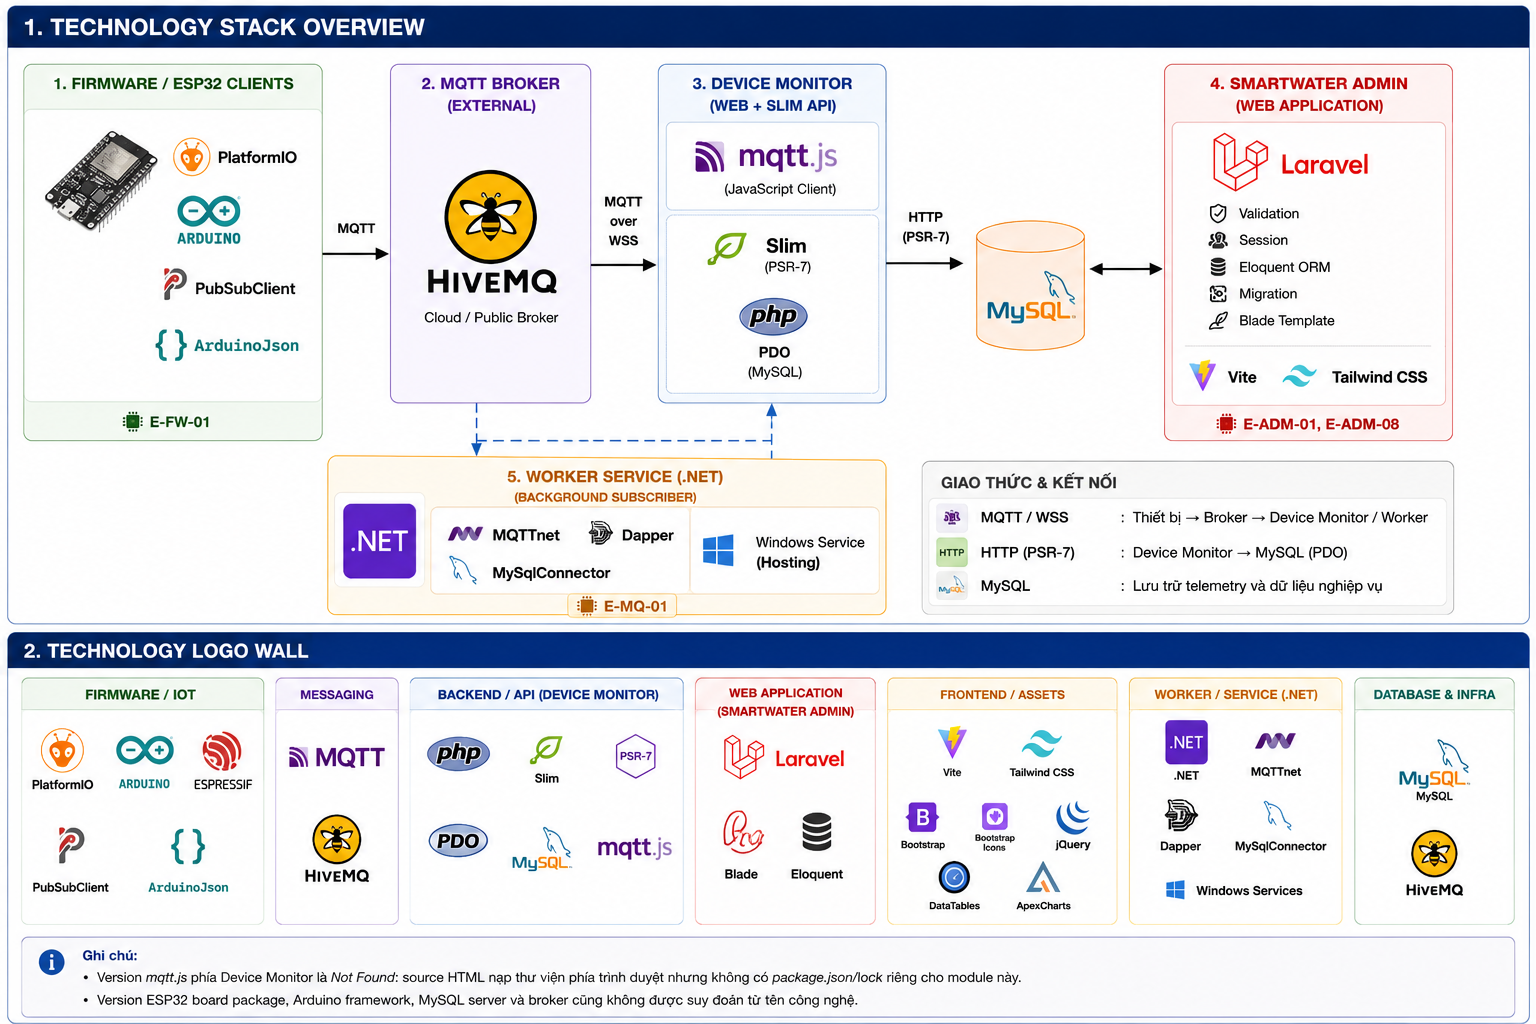
\includegraphics[width=0.8\textwidth]{include/images/tech_framework.png}
    \caption{Technology Stack Overview của hệ thống SmartWater}
    \label{fig:tech-framework}
\end{figure}
```
